本节将给出程序在模拟器上的运行结果与分析。
\subsection{初始化界面}
为了简约化,这里将背景色统一设置为绿色,障碍物颜色设置为蓝色,坦克和子弹的颜色则为红色。下图展示了初始化界面,包括一辆红色的坦克和一个刚产生的障碍物。\\

\begin{figure}[H]
  \centering
  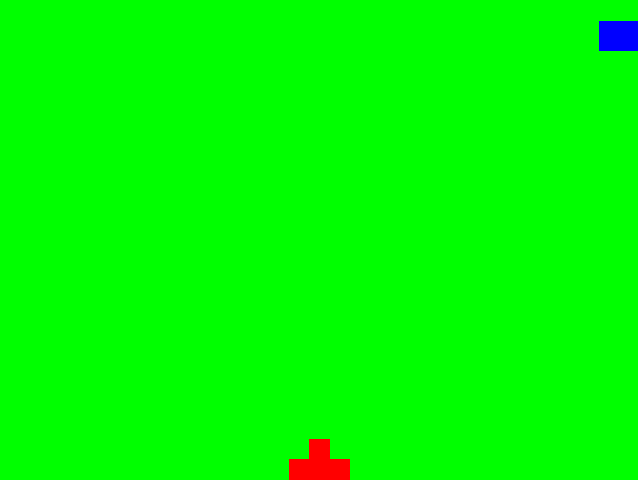
\includegraphics[width=0.7\textwidth]{img/init.png}
  \caption{初始化界面
  }\label{fig:init}
\end{figure}

\subsection{障碍物随机增加和坦克移动}
这里随着程序继续运行,障碍物将会随机产生,并不断往下坠落。坦克可以上下左右自由移动,并选择时机发生子弹。下图展示了运行一段时间后的界面,此时障碍物的数量增加,坦克进行了一定的位移。\\

\subsubsection{坦克移动}
\begin{figure}[H]
  \centering
  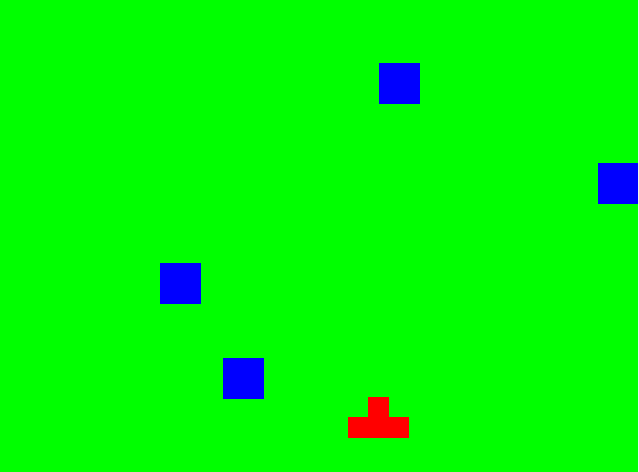
\includegraphics[width=0.7\textwidth]{img/later.png}
  \caption{一段时间后的界面
  }\label{fig:later}
\end{figure}

\subsubsection{障碍物出界,游戏结束}
由于出界时,尚未击中任何障碍物,因此得分为负,游戏结束。
\begin{figure}[H]
  \centering
  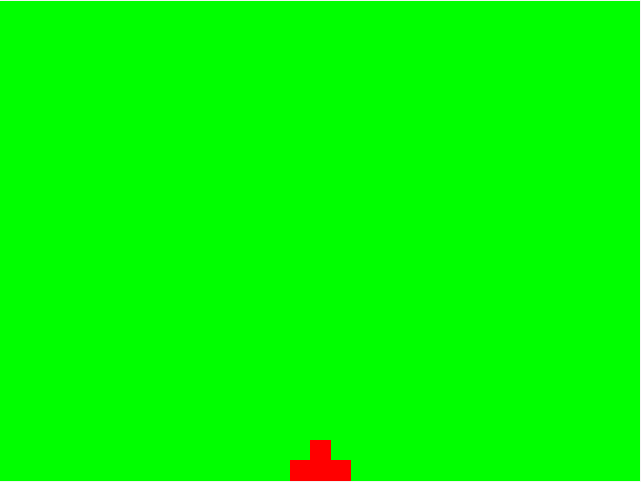
\includegraphics[width=0.7\textwidth]{img/new.png}
  \caption{重新初始化界面
  }\label{fig:new}
\end{figure}

\subsection{坦克发射子弹的过程}
为了避免障碍物坠落到边界以下,坦克需要发射子弹来消灭障碍物。下面的几张图演示了子弹发射前后的过程。\\

\subsubsection{子弹在坦克内上膛的过程}
\begin{figure}[H]
  \centering
  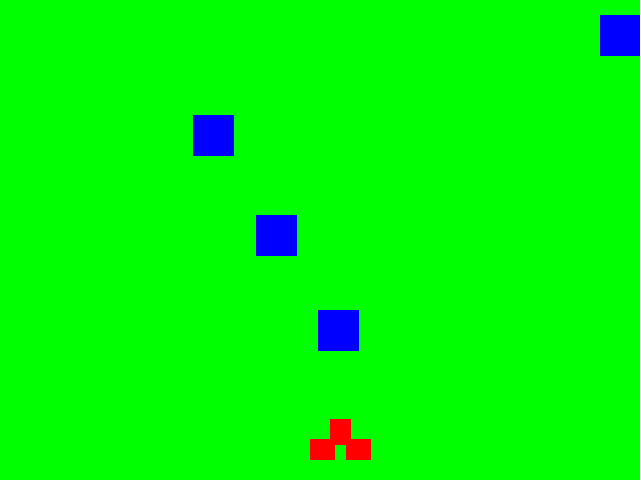
\includegraphics[width=0.7\textwidth]{img/shot1.png}
  \caption{子弹上膛
  }\label{fig:shot1}
\end{figure}

\subsubsection{子弹发射之后的状态}
\begin{figure}[H]
  \centering
  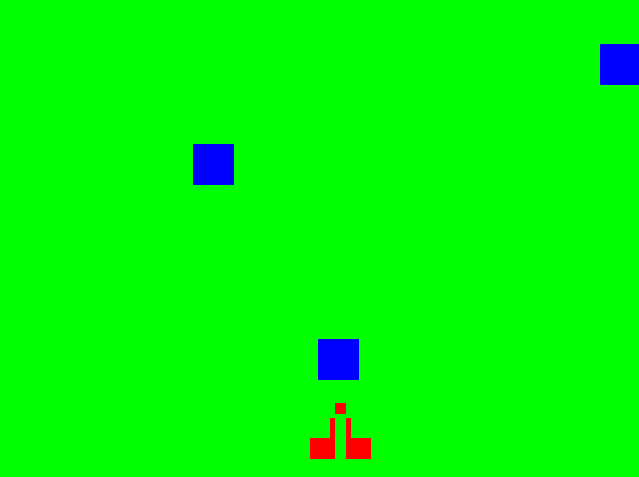
\includegraphics[width=0.7\textwidth]{img/shot2.png}
  \caption{子弹发射后
  }\label{fig:shot2}
\end{figure}

\subsubsection{子弹即将击中障碍物}
\begin{figure}[H]
  \centering
  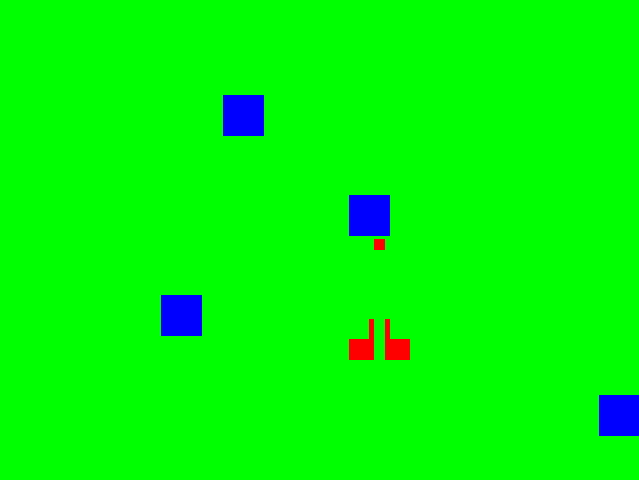
\includegraphics[width=0.7\textwidth]{img/shot3.png}
  \caption{即将击中障碍物
  }\label{fig:shot3}
\end{figure}

\subsubsection{击中障碍物后}
\begin{figure}[H]
  \centering
  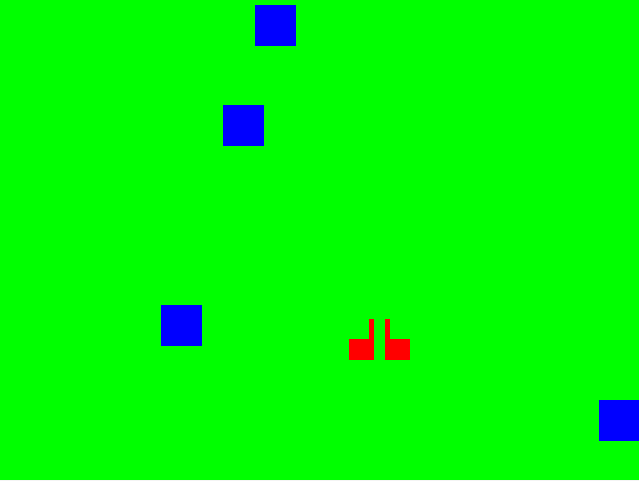
\includegraphics[width=0.7\textwidth]{img/shot4.png}
  \caption{击中障碍物后,子弹与障碍物同时消失
  }\label{fig:shot4}
\end{figure}

\subsubsection{坦克继续移动}
\begin{figure}[H]
  \centering
  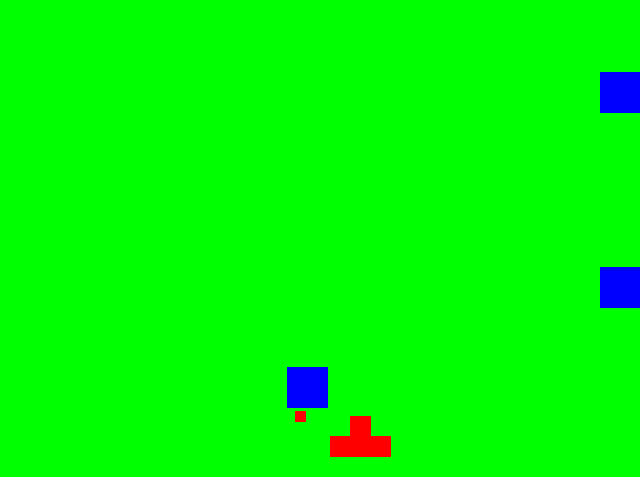
\includegraphics[width=0.7\textwidth]{img/shot5.png}
  \caption{发射子弹后,坦克继续移动
  }\label{fig:shot5}
\end{figure}

\subsection{七段数码管显示得分情况}
七段数码管的前四个显示历史最高分,后四个显示当前得分。当坦克击中障碍物时加1分,当障碍物超出下边界时扣2分。当用户分数为负,或坦克与障碍物相撞时,游戏结束。下图中,当前得分为2分,历史最高分为7分。\\

\begin{figure}[H]
  \centering
  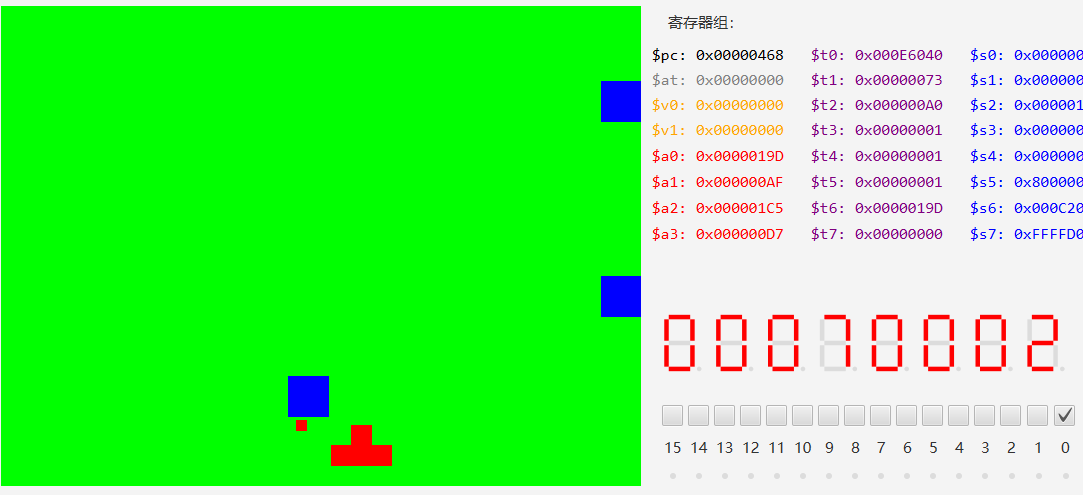
\includegraphics[width=0.8\textwidth]{img/score.png}
  \caption{七段数码管显示得分情况
  }\label{fig:score}
\end{figure}



